
\documentclass{standalone}
\usepackage{amsthm,amsmath,amssymb}
\usepackage{amsfonts}
\usepackage{tikz}
\usetikzlibrary{positioning, shapes.geometric}
\usetikzlibrary{calc}

% Define the basic shape of flow chart
\tikzstyle{startstop} = [rectangle, rounded corners, minimum width = 2cm, minimum height=1cm,text centered, draw = black, fill = red!30]
\tikzstyle{io} = [trapezium, trapezium left angle=70, trapezium right angle=110, minimum width=2cm, minimum height=1cm, text centered, draw=black, fill = blue!25]
\tikzstyle{process} = [rectangle, minimum width=3cm, minimum height=1cm, text centered, draw=black, fill = yellow!35]
\tikzstyle{decision} = [diamond, aspect = 3, text centered, minimum width = 2.5cm, draw=black, fill = green!45]
% arrow shape
\tikzstyle{arrow} = [->,>=stealth]

\begin{document}

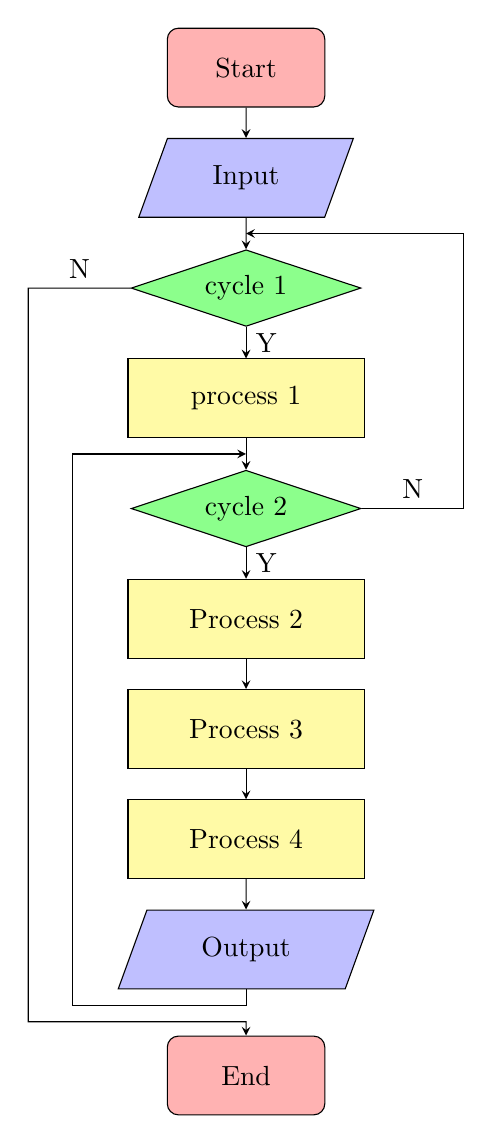
\begin{tikzpicture}[node distance = 1.2cm]
  % Define flowchart  shape
  \node (start) [startstop] {Start};
  \node (in1) [io, below of = start, yshift=-0.2cm, minimum width=1cm] {Input};
  \node (dec1) [decision, below of=in1, yshift=-0.2cm] {cycle 1};
  \node (pro1) [process, below of=dec1,yshift=-0.2cm] {process 1};
  \node (dec2) [decision, below of=pro1, yshift=-0.2cm] {cycle 2};
  \node (pro2) [process, below of=dec2,yshift=-0.2cm] {Process 2};
  \node (pro3) [process, below of=pro2,yshift=-0.2cm] {Process 3};
  \node (pro4) [process, below of=pro3,yshift=-0.2cm] {Process 4};
  \node (in2)  [io, below of=pro4, yshift=-0.2cm] {Output};
  \node (stop) [startstop, below of=in2,node distance = 1.6cm] {End};
  % connect
  \draw[arrow] (start)  -- (in1);
  \draw[arrow] (in1) -- (dec1);
  \draw[arrow] (dec1.west)-- node[anchor=south] {N} ($(dec1.west) - (1.3,0)$) |- ($(stop.north)!.3!(in2.south)$) -- (stop);
  \draw[arrow] (dec1) -- node[anchor=west] {Y} (pro1);
  \draw[arrow] (pro1) -- (dec2);
  \draw[arrow] (dec2.east) -- node[anchor=south] {N} ($(dec2.east) + (1.3,0)$) |- ($(in1.south)!.5!(dec1.north)$);
  \draw[arrow] (dec2) -- node[anchor=west] {Y} (pro2);
  \draw[arrow] (pro2) -- (pro3);
  \draw[arrow] (pro3) -- (pro4);
  \draw[arrow] (pro4) -- (in2);
  \draw[arrow] (in2.south)  -- ($(in2.south)-(0,0.2)$) -- ($(in2.south) - (2.2,0.2)$) |- ($(pro1.south)!.5!(dec2.north)$);
\end{tikzpicture}

\end{document}